\textbf{See the instruction for questions \inteval{\value{question}+1} to \inteval{\value{question}+2}.}

\begin{center}
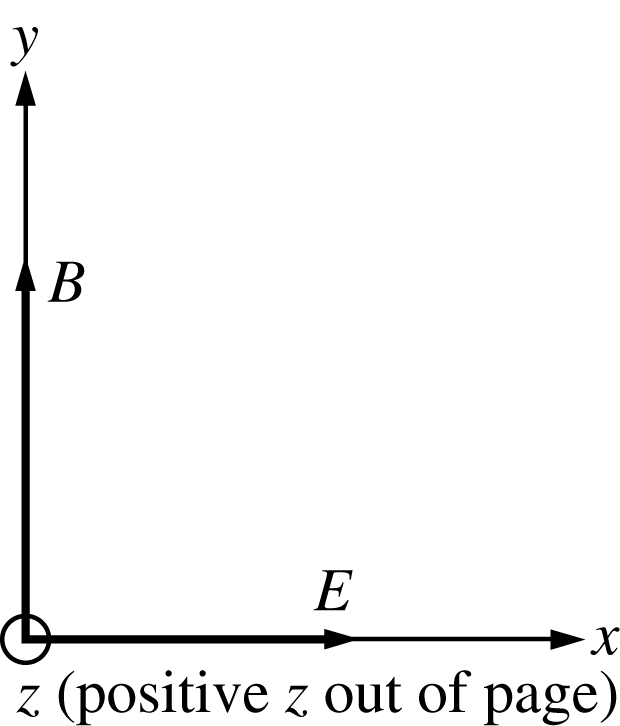
\includegraphics[scale=0.2]{images/img-004-004.png}
\end{center}

A region contains a uniform electric field of strength $E$ in the $+x$-direction and a uniform magnetic field of strength $B$ in the +$y$-direction, relative to the axes shown above. A positively charged particle passes through these two fields in a straight line at a constant speed $v$.

% Multiple Choice Question 6
\begin{questions}\setcounter{question}{5}\question
The velocity of the particle is in which direction?

\begin{oneparchoices}
\choice $+y$
\choice $+x$
\choice $-x$
\choice $+z$
\choice $-z$
\end{oneparchoices}\end{questions}

% Multiple Choice Question 7
\begin{questions}\setcounter{question}{6}\question
The magnetic field strength $B$ is equal to

\begin{oneparchoices}
\choice $E$
\choice $E v$
\choice $\dfrac{E}{v}$
\choice $\dfrac{v}{E}$
\choice $E v^{2}$
\end{oneparchoices}\end{questions}

